\documentclass[12pt,a4paper,titlepage]{scrreprt}
\usepackage[utf8]{inputenc}
%\usepackage{amsmath}	%sonst für Mathe zustädnig
\usepackage{mathpazo} 	%für das |R etc. Mathemodus
\usepackage{commath}
\usepackage{IEEEtrantools}
\usepackage{siunitx}
%textart aendern
\usepackage[varg]{txfonts}
\usepackage{enumitem}
\usepackage{graphicx}
\usepackage{caption}
\usepackage{empheq}    % lädt »mathtools«, welches wiederum »amsmath« lädt
\usepackage{subcaption}
\usepackage{float} %erzwingt ort der Figure
\usepackage{amsfonts}
\usepackage{amssymb}
\usepackage{multirow}	%Multirow
\usepackage{graphicx}
\usepackage{xcolor}
\usepackage{cancel}
\usepackage{arydshln}	%für Gepunktete Linien bei tabellen
\usepackage[ngerman]{babel}
\usepackage[autostyle=true]{csquotes}
\usepackage{hyperref}
\graphicspath{{figs/}}
\usepackage{edv_makros}
\author{Kilian Kranz \& Achim Bruchertseifer}
\title{Treibhauseffekt}
\subtitle{Übungsblatt 3 zur Vorlesung \glqq Computerphysik\grqq~ SS 2018}
\begin{document}
	\maketitle
	\setcounter{chapter}{3}

	\section{Problemstellung}
	Der Treibhauseffekt soll an einem einfachen Modell untersucht werden, indem die mittlere Temperatur der Erde $T_E$ durch eine nichtlineare Gleichung berechnet wird. Das betrachtete System wird in einen Gleichgewichtszustand angenommen und über die drei Gleichgewichte des Strahlungsverhaltens von der Atmosphäre, der Sonne und der Erde selbst kann die entscheidende Gleichung entzogen werden:
	\begin{align}
		\left[2-\epsilon\left(T_E\right)\right]\cdot T_E^4=&~\epsilon_S\left[2-\epsilon\left(T_S\right)\right]\cdot T_S^4~~.	\label{31}
	\end{align}
	Hier ist $\epsilon_S$ die effektive Emissivität der Sonne und $\epsilon\left(T\right)$ die der Atmosphäre in Abhängigkeit der Temperatur:
	\begin{align}
	\epsilon(T)=&~\dfrac{1}{Z}\underbrace{\int\limits_0^\infty~\rho\left(\nu,T\right)\cdot\left[1-f(\nu\right]~\dif\nu}_{\text{numerischer Teil}}~,~~~~Z=\underbrace{\int\limits_0^\infty~\rho\left(\nu,T\right)~\dif\nu}_{\text{analytischer Teil}}~~.
	\end{align}
	Diese zwei Gleichungen stellen den Kern des Problems da. Gesucht ist die Gleichgewichtstemperatur der Erde, $T_E$, in Abhängigkeit von $\tilde{n}$, das die Luftsäulendichte als Anteil von $N$ beschreibt.	
	
	\section{Lösung des Problems}
	\subsection{Lösung des analytischen Integrals}
	Über eine \textsc{Taylor}entwicklung über den Ausdruck $\dfrac{1}{\euler^x-1}$ ergibt sich mittels Partieller Integration:
	\begin{align}
		Z=&~\sum_{m}^{\infty}\dfrac{48\pi~k^4}{c^3~h^3~m^4}~T^4~~.
	\end{align}
	Dies kann nun bis zu einer bestimmten Genauigkeit implementiert werden.
	
	\subsection{Lösung des numerischen Integrals}
	Mithilfe der \textsc{Simpson}schen Regel kann der numerische Teil von $\epsilon(T)$ über eine gerade Anzahl von $n$ Stützstellen berechnet werden.
	(verarbeitet in den Funktionen\textit{ \glqq Simpson\_Fkt\grqq}~und \textit{\glqq Integral\_S\grqq})
	\begin{align}
		\int\limits_a^b~f(x)~\dif x =&~\dfrac{h}{3}\left(f_a+4f_1+2f_2+4f_3+\dots+4f_{n-1}+f_b\right)+\mathcal{O}\left(h^4\right)~~,
	\end{align}
	wobei $h=\dfrac{b-a}{n}$ die Schrittweite ist.
	
	\subsection{Lösung der nichtlinearen Gleichung}
	Die nichtlineare Gleichung \eqref{31} lässt sich umformen zu
	\begin{align}
		T_E=&~T_S\sqrt[4]{\dfrac{\epsilon_S\cdot\left(2-\epsilon\left(T_S\right)\right)}{2-\epsilon\left(T_E\right)}}~~.
	\end{align}
	Nun kann man über den Fixpunktansatz rekursiv ($x_{k+1}=T_E(x_k)$)  eine Näherung für die Gleichung bestimmen. (siehe Funktion \textit{\glqq Fixpunkt\grqq})
		

	\section{Ergebnis}
	Gefordert war die Lösung des Problems explizit für $\tilde{n}=1$, welches für  $T_E=$\underline{$25.45^\circ$C} ergibt. Dieser Wert passt gut in die Erwartung, da mit diesen Werten die Anzahl der CO$_2$-Moleküle den momentanen Stand darstellen. Größere Werte von $\tilde{n}$ beschreiben das Fortschreiten des Treibhauseffektes; dies ergibt eine konvergierende Kurve, welche in \figureref{B1} zu finden ist.

	
	\section{Anhang}
	\begin{figure}[H]
		\flushleft
		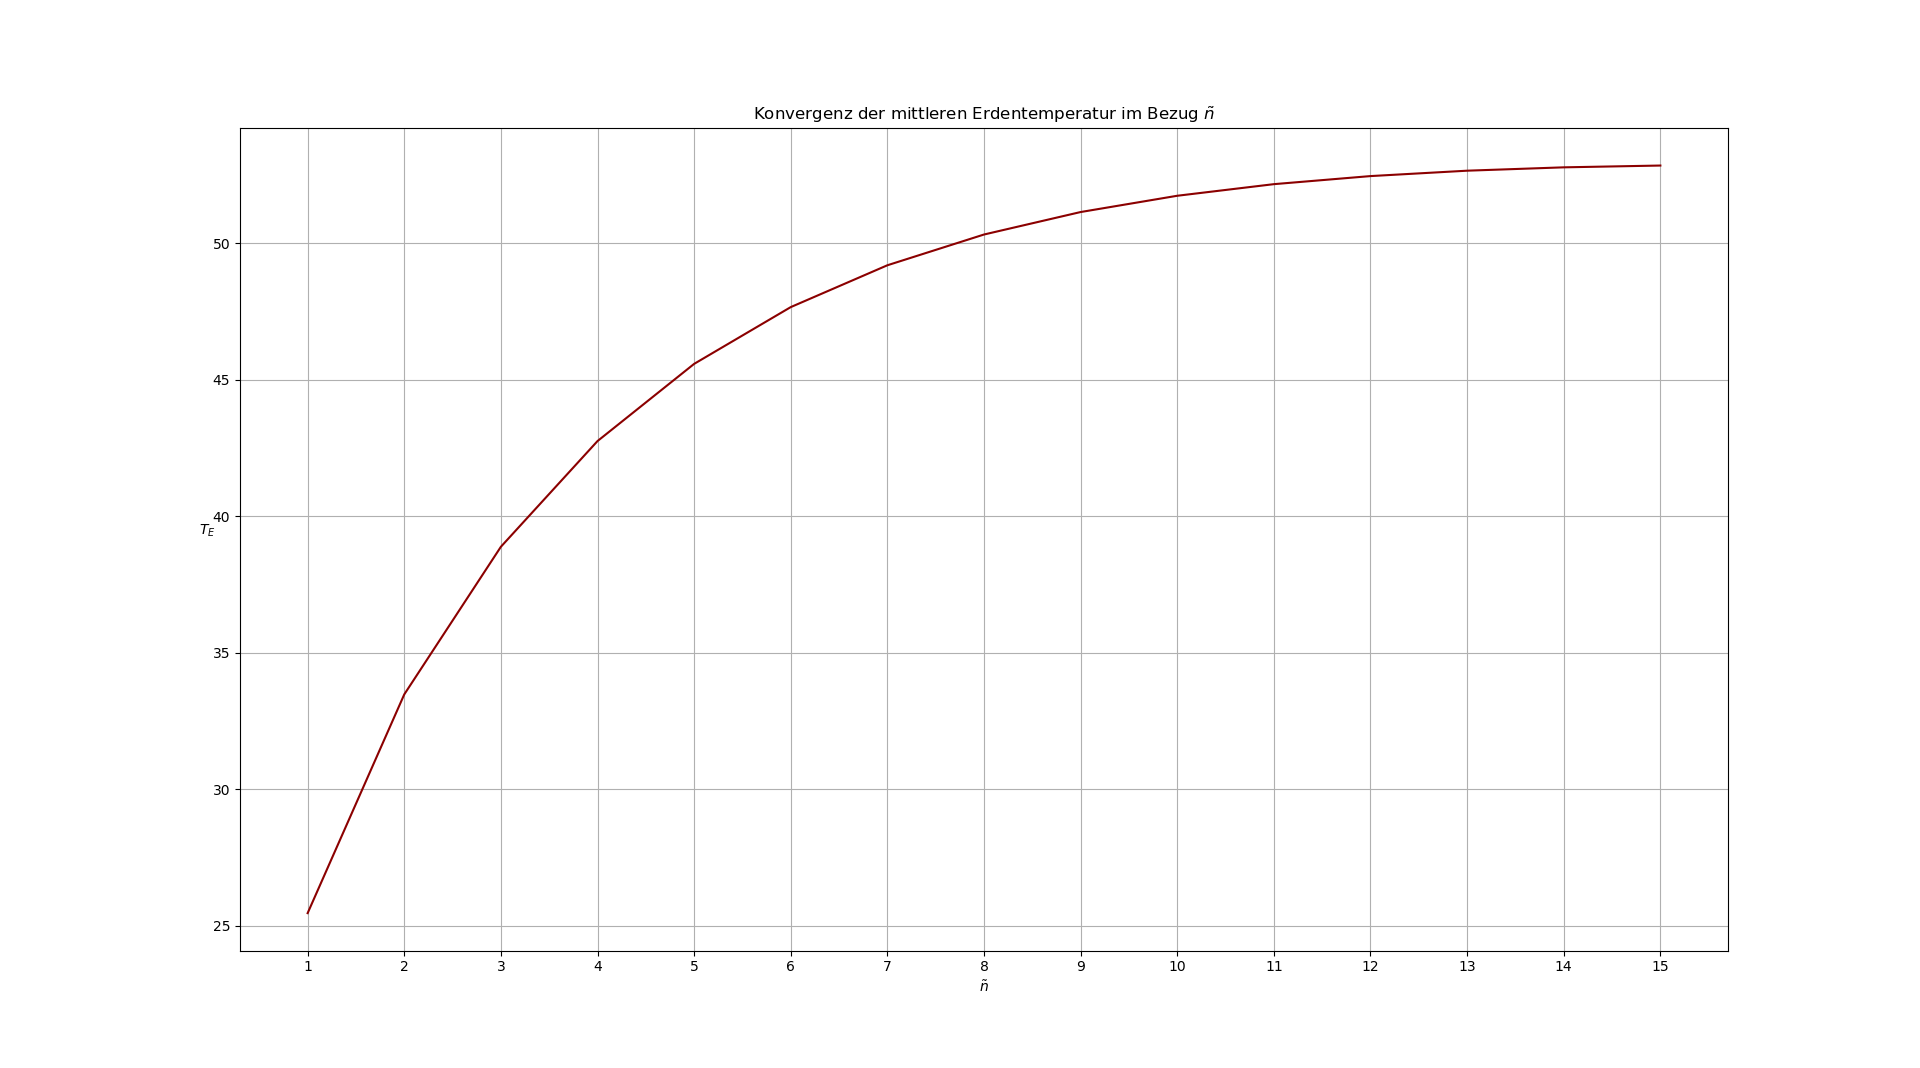
\includegraphics[width=1\textwidth]{Konvergenz}
		\caption{Konvergenz der nichtlinearen Gleichung für wachsende $\tilde{n}$. Mit Werten: \tableref{T1}.}
		\label{B1}
	\end{figure}

	\begin{table}[H]
		\centering
		\begin{tabular}{l|l}
			\textbf{$T_E$}&\textbf{$\tilde{n}$}\\\hline
				25.4529162&1\\
				33.4676782&2\\
				38.8769997&3\\
				42.7499765&4\\
				45.5783748&5\\
				47.6588755&6\\
				49.1915598&7\\
				50.3182622&8\\
				51.1419588&9\\
				51.7383605&10\\
				52.163556&11\\
				52.4593226&12\\
				52.6569166&13\\
				52.7798176&14\\
				52.8457325&15 
		\end{tabular}
	\caption{Zugehörigen Werte zum Plot}
	\label{T1}
	\end{table}
	
\end{document}